
\chapter{Die Mathematik der Natur}

% =====================================================
% 10.1 Einleitung: Sichtbare Natur, verborgene Ordnung
% =====================================================
\subsection{Einleitung: Sichtbare Natur, verborgene Ordnung}

Wer an Mathematik denkt, denkt oft an Zahlen, Formeln und abstrakte Begriffe. Die Natur dagegen erscheint zunächst anders: vielfältig, unregelmäßig, lebendig und oft schwer berechenbar. Bäume wachsen nicht wie ideale Linien, Wolken haben keine exakten Konturen, Flüsse folgen keinem Lineal, und selbst Blüten oder Kristalle zeigen zwar Ordnung, aber nie in der vollkommenen Reinheit eines Lehrbuchbildes. Gerade deshalb scheint die sichtbare Welt auf den ersten Blick eher das Gegenteil mathematischer Strenge zu sein.

Doch dieser Eindruck täuscht. Hinter der Vielfalt der Natur verbergen sich häufig Strukturen, die sich mathematisch beschreiben lassen. Diese Struktur zeigt sich nicht immer in vollkommener Regelmäßigkeit, sondern oft in wiederkehrenden Mustern, in funktionalen Kompromissen, in Symmetrien, Wachstumsprozessen oder energetisch günstigen Formen. Die Mathematik der Natur liegt daher nicht nur in idealen Figuren, sondern gerade in den Gesetzmäßigkeiten, die reale Formen hervorbringen.

So entstehen Bienenwaben nicht als dekorative Muster, sondern als effiziente Struktur mit geringem Materialaufwand. Verzweigungen bei Bäumen, Blutgefäßen oder Flusssystemen folgen nicht bloß zufälligem Wachstum, sondern funktionalen Anforderungen an Versorgung, Stabilität und Transport. Schneeflocken und Kristalle zeigen Symmetrien, die aus den Eigenschaften ihrer mikroskopischen Bausteine hervorgehen. Spiralen in Pflanzen oder Muster auf Tierfellen entstehen aus lokalen Regeln, die im Zusammenspiel eine sichtbare Ordnung hervorbringen.

In all diesen Fällen beschreibt Mathematik nicht einfach etwas, das man ohnehin schon vollständig verstanden hätte. Sie macht vielmehr präzise sichtbar, welche Struktur hinter den Formen wirkt. Sie zeigt, warum bestimmte Gestalten bevorzugt auftreten, welche Bedingungen ihr Wachstum lenken und weshalb sich aus vielen Möglichkeiten gerade einige wenige stabile oder effiziente Muster durchsetzen. Mathematik ist hier nicht bloß Sprache, sondern Erkenntnisinstrument.

Zugleich darf man die Natur nicht mit einem idealisierten Lehrbuch verwechseln. Reale Systeme sind unvollkommen, gestört, historisch gewachsen und von vielen Einflüssen geprägt. Gerade deshalb ist es wichtig, zwischen mathematischem Modell und konkreter Wirklichkeit zu unterscheiden. Die Mathematik erfasst nicht jedes Detail, aber sie legt Ordnungen frei, die im scheinbar Zufälligen verborgen sind.

Dieses Kapitel führt deshalb bewusst zurück zur sichtbaren Welt. Nach den historischen, philosophischen und modernen Perspektiven der vorangegangenen Kapitel soll nun an konkreten Beispielen gezeigt werden, wie mathematische Struktur in der Natur hervortritt. Es geht nicht darum, die Wirklichkeit auf Formeln zu reduzieren, sondern sichtbar zu machen, dass Naturformen, Wachstumsprozesse und Ordnungen oft einem mathematisch beschreibbaren Zusammenhang folgen. Gerade darin bestätigt sich erneut der Leitgedanke dieses Buches: Die Welt ist nicht mathematisch dekoriert, sondern mathematisch strukturiert.

\begin{DidacticBox}[Natur und mathematische Struktur]
	Mathematik zeigt sich in der Natur nicht nur in perfekten Formen, sondern auch in Wachstumsprozessen, Symmetrien, Optimierungen und wiederkehrenden Mustern. Gerade dort, wo die sichtbare Welt unregelmäßig erscheint, kann mathematische Beschreibung die verborgene Ordnung sichtbar machen.
\end{DidacticBox}
% =====================================================
% 10.2 Bienenwaben und das Prinzip der optimalen Form
% =====================================================

\subsection{Bienenwaben und das Prinzip der optimalen Form}
\index{Bienenwabe}
\index{Geometrie}
\index{Leichtbau}
\index{Optimierung}
\index{Honeycomb-Struktur}

Bienenwaben sind ann\"ahernd sechseckig. Das ist keine blo{\ss}e dekorative Form, sondern Ausdruck geometrischer Effizienz. Regelm\"a{\ss}ige Sechsecke k\"onnen eine Fl\"ache l\"uckenlos f\"ullen und ben\"otigen dabei bei gegebener Zellgr\"o{\ss}e nur wenig Wandl\"ange. Dadurch entsteht eine Struktur, die mit geringem Materialeinsatz eine gro{\ss}e Zahl stabiler Zellen bereitstellt.

Gerade darin zeigt sich ein grundlegendes mathematisches Prinzip: Unter gegebenen Bedingungen setzt sich nicht irgendeine Form durch, sondern eine, die bestimmte Anforderungen besonders gut erf\"ullt. Im Fall der Bienenwabe geht es um einen Kompromiss aus Stabilit\"at, Platzausnutzung und Materialersparnis. Die sechseckige Struktur ist daher keine zuf\"allige Laune der Natur, sondern eine Form, die sich funktional bew\"ahrt.

Dasselbe Prinzip findet sich auch in der Technik. Im Leichtbau, besonders in der Luft- und Raumfahrt, werden sogenannte Wabenkerne als Kern von Sandwich-Bauteilen verwendet. Zwei d\"unne, feste Decklagen werden durch einen leichten Kern auf Abstand gehalten. Der Wabenkern stabilisiert gegen Beulen und nimmt Schubkr\"afte auf, w\"ahrend die Decklagen bei Biegung Zug- und Druckkr\"afte tragen. So entsteht eine sehr hohe Biegesteifigkeit bei geringem Gewicht.

Damit wird sichtbar, dass dieselbe geometrische Idee in Natur und Technik wirksam ist. Was im Bienenstock als nat\"urliche Struktur erscheint, wird im Ingenieurwesen bewusst als Konstruktionsprinzip genutzt. Mathematik zeigt sich hier nicht nur als Beschreibung einer vorhandenen Form, sondern als Einsicht in ein Ordnungsprinzip, das sich praktisch anwenden l\"asst.

\begin{NoteBox}[Die Biene rechnet nicht -- aber die Struktur entsteht]
	\small
	Die Wabe zeigt, dass mathematische Struktur nicht erst im menschlichen Denken beginnt. Wenn Material, Kr\"afte und Randbedingungen zusammenwirken, entstehen in der Natur oft stabile geometrische Formen. Mathematik ist dann nicht blo{\ss} Erfindung, sondern das pr\"azise Instrument, mit dem wir solche Strukturen erkennen, beschreiben und technisch nutzen -- vom Bienenstock bis zur Sandwichstruktur im Leichtbau.
\end{NoteBox}

\begin{figure}[htbp]
	\centering
	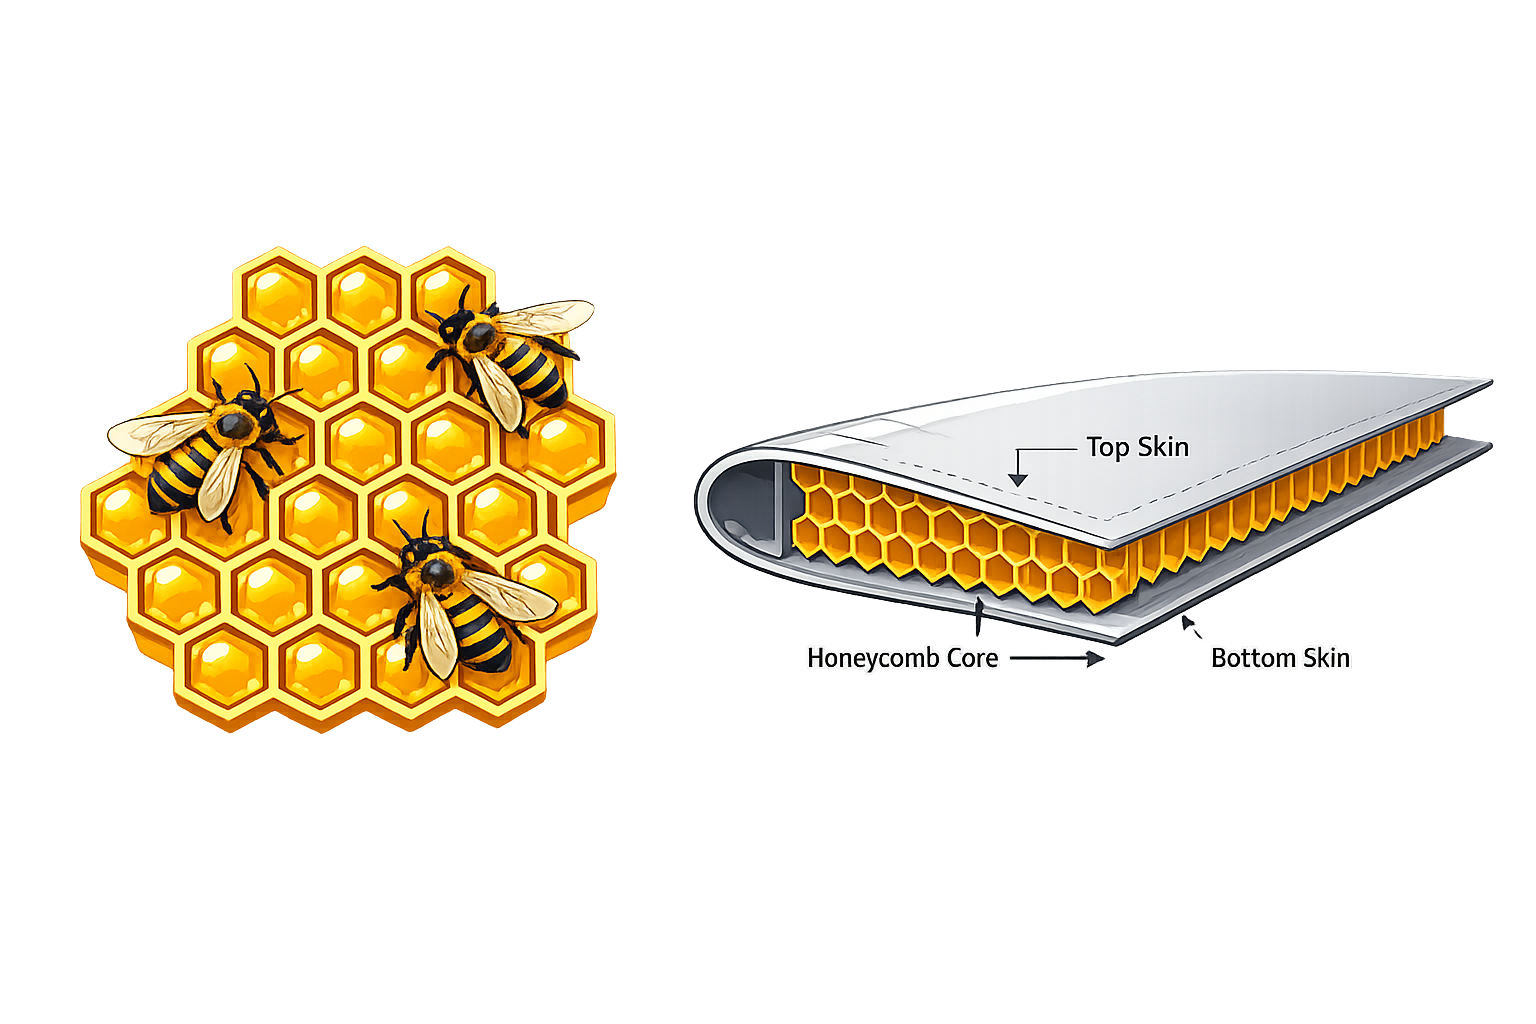
\includegraphics[width=0.85\linewidth]{bilder/Bienen.png}
	\caption{Bienenwaben und technischer Leichtbau: dieselbe Strukturidee in Natur und Technik.}
	\label{fig:waben_leichtbau}
\end{figure}
\newpage
\noindent

% =====================================================
% 10.3 Verzweigungsnetzwerke in Natur und Technik
% =====================================================

\subsection{Verzweigungsnetzwerke in Natur und Technik}
\index{Verzweigung}
\index{Netzwerk}
\index{Baum}
\index{Biologie}
\index{Optimierung}
\index{Stringtheorie}
\index{Minimalfl\"achen}

Verzweigungsnetzwerke geh\"oren zu den eindrucksvollsten Formen nat\"urlicher Ordnung. Sie finden sich in B\"aumen, Wurzelsystemen, Blutgef\"a{\ss}en, Bronchien, Flusssystemen oder Nervenzellen. Auf den ersten Blick wirken solche Strukturen oft unregelm\"a{\ss}ig. Bei genauerem Hinsehen zeigen sie jedoch ein wiederkehrendes Prinzip: Ein Hauptstrang teilt sich in kleinere Einheiten auf, die ihrerseits weiter verzweigt sind. So entsteht ein Netzwerk, das Versorgung, Transport oder Verteilung mit m\"oglichst geringem Aufwand erm\"oglicht.

Ein anschauliches Beispiel liefert die Botanik. Ein Baum maximiert mit seiner Krone die Aufnahme von Licht, muss aber zugleich Wasser und N\"ahrstoffe \"uber ein verzweigtes Leitungsnetz bis in gro{\ss}e H\"ohen transportieren. Die entstehende Form ist daher kein Zufall, sondern das Ergebnis eines Kompromisses zwischen Wachstum, Versorgung, Materialaufwand und mechanischer Stabilit\"at. Genau solche Zielkonflikte lassen sich mathematisch als Optimierungsprobleme beschreiben.

\begin{DidacticBox}[Nicht Zufall, sondern funktionale Struktur]
	\label{box:verzweigungsnetzwerk}
	Verzweigungsformen in der Natur entstehen nicht deshalb, weil ein Organismus \glqq rechnet\grqq. Sie entstehen, weil Transport, Stabilit\"at, Materialeinsatz und Wachstum gleichzeitig erf\"ullt werden m\"ussen. Mathematik macht diese Zielkonflikte sichtbar und beschreibt, warum bestimmte Netzwerkformen unter gegebenen Bedingungen besonders g\"unstig sind.
\end{DidacticBox}

Solche Netzwerke sind nicht nur biologisch interessant, sondern auch technisch bedeutsam. Dieselben Fragen treten in Leitungsnetzen, Verkehrswegen, Rohrsystemen oder Versorgungsstrukturen auf: Wie kann etwas effizient verteilt werden, ohne unn\"otig Material, Energie oder Platz zu verbrauchen? Gerade hier zeigt sich, dass mathematische Begriffe wie Optimierung, Netzwerkstruktur und Minimalit\"at nicht an ein bestimmtes Material gebunden sind, sondern an die Form der Beziehungen selbst.

Im 21.~Jahrhundert ist dieser Methodentransfer besonders fruchtbar geworden. Mathematische Werkzeuge, die urspr\"unglich in sehr abstrakten Gebieten entwickelt wurden, finden heute Anwendung in realen Netzwerkproblemen. So k\"onnen Methoden aus der Theorie von Minimalfl\"achen, geometrischer Optimierung oder sogar aus dem Umfeld der Stringtheorie genutzt werden, um die Geometrie verzweigter R\"ohrennetzwerke zu untersuchen. Gemeint ist dabei nicht, dass ein Baum oder ein Blutgef\"a{\ss} \glqq aus Strings\grqq\ best\"unde. Entscheidend ist vielmehr, dass sich in ganz unterschiedlichen Zusammenh\"angen dieselben mathematischen Strukturprobleme wiederfinden.

Gerade darin zeigt sich die Reichweite mathematischen Denkens. Ein Verzweigungsnetzwerk ist nicht nur ein biologisches oder technisches Objekt, sondern ein Beispiel daf\"ur, dass die Natur auf wiederkehrende Weise Probleme von Versorgung, Stabilit\"at und Effizienz l\"ost. Mathematik beschreibt hier nicht blo{\ss} eine sichtbare Form, sondern die verborgene Ordnung, die diese Form hervorbringt. Eine ausf\"uhrlichere mathematische Behandlung eines solchen Verzweigungsnetzwerks folgt in Anhang~\ref{app:netzwerke-minimalflaeche}.

\begin{figure}[htbp]
	\centering
	
\includegraphics[width=0.62\linewidth]{bilder/Baum.png}
	\caption{Verzweigungsstruktur eines jungen Baumes. Sichtbar wird hier nicht nur eine botanische Form, sondern ein nat\"urliches Netzwerk, dessen Gestalt als Kompromiss zwischen Wachstum, Versorgung und Stabilit\"at verstanden werden kann.}
	\label{fig:baum-verzweigung}
\end{figure}

\newpage
\noindent

% =====================================================
% 10.4 Spiralen und Blattstellungen bei Pflanzen
% =====================================================


\subsection{Spiralen und Blattstellungen bei Pflanzen}
\index{Spirale}
\index{Blattstellung}
\index{Pflanze}
\index{Fibonacci-Folge}
\index{Phyllotaxis}
\index{Wachstum}
\index{Optimierung}

Auch in der Pflanzenwelt zeigt sich Mathematik nicht nur in idealen Figuren, sondern in realen Wachstumsprozessen. Besonders auffällig ist dies bei Spiralen und Blattstellungen. Blätter sitzen oft nicht zufällig am Stängel, sondern in einer Anordnung, die verhindert, dass sie sich gegenseitig zu stark beschatten. Ähnliche Muster finden sich in Sonnenblumen, Tannenzapfen, Ananasfrüchten oder Kakteen, wo Samen, Schuppen oder Blätter in deutlich erkennbaren Spiralstrukturen angeordnet sind.

Solche Anordnungen werden in der Botanik unter dem Begriff \emph{Phyllotaxis} zusammengefasst. Gemeint ist damit die gesetzmäßige Stellung von Blättern, Knospen oder anderen Pflanzenteilen entlang einer Wachstumsachse. Mathematisch interessant wird dies deshalb, weil aus einfachen lokalen Wachstumsregeln überraschend geordnete Gesamtmuster entstehen. Neue Blätter oder Samen erscheinen jeweils an Positionen, die bereits vorhandenen Strukturen ausweichen. Dadurch wird der verfügbare Raum möglichst gleichmäßig genutzt.

Besonders bekannt ist in diesem Zusammenhang der Bezug zur Fibonacci-Folge. 

\begin{NoteBox}[Fibonacci und Pflanzen]
	Die Fibonacci-Zahlen erscheinen in Pflanzen nicht als bewusstes Rechenverfahren, sondern als Folge bestimmter Wachstums- und Packungsregeln. Eine kurze mathematische Erläuterung findet sich in Anhang~\ref{app:fibonacci-goldener-schnitt}.
\end{NoteBox}
\newpage
\noindent
Wie in Abbildung~\ref{fig:sunflower-fibonacci} zu sehen ist, entstehen bei Sonnenblumen geordnete Spiralstrukturen, die häufig mit Fibonacci-Zahlen in Verbindung stehen.
\begin{figure}[htbp]
	\centering
	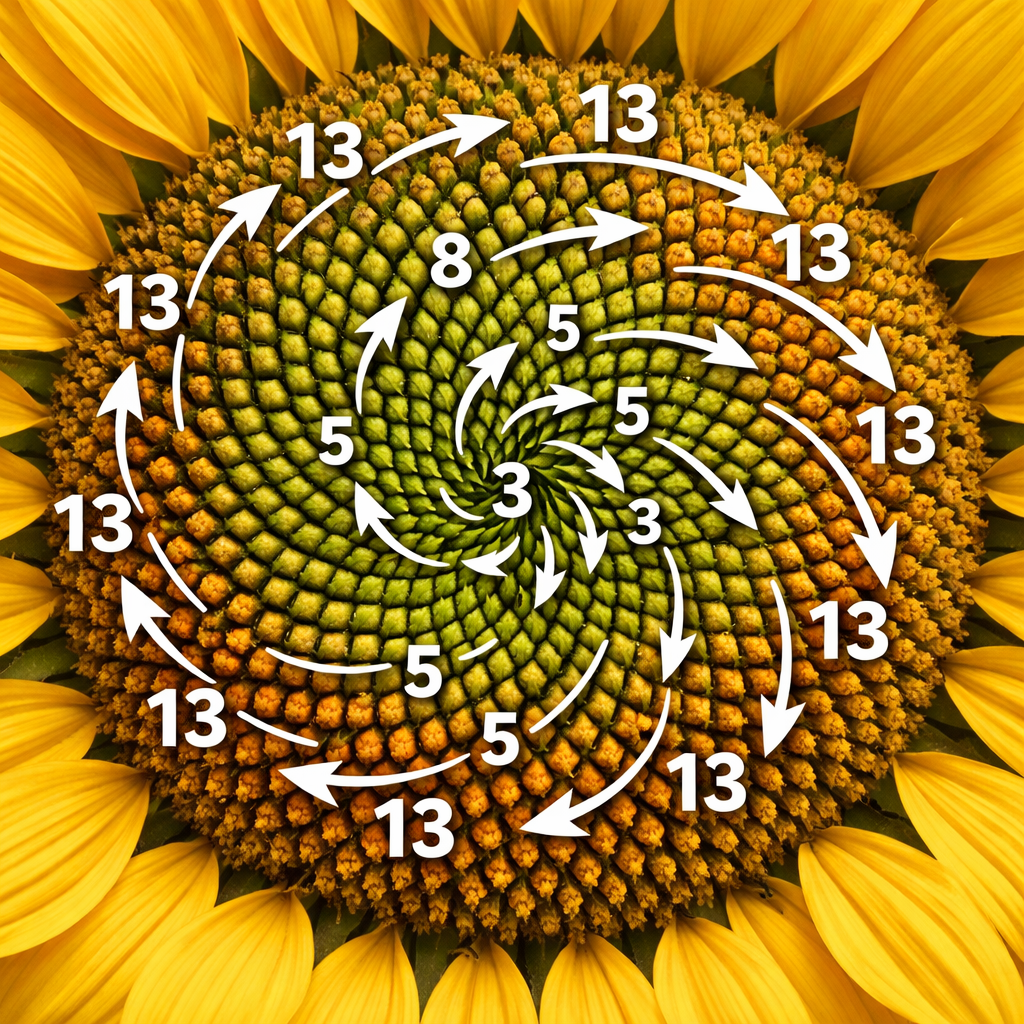
\includegraphics[width=0.82\linewidth]{bilder/sunflower.png}
	\caption{Sonnenblume mit sichtbaren Spiralstrukturen. Solche Anordnungen stehen im Zusammenhang mit Wachstumsregeln und effizienter Platzverteilung; dabei treten häufig Spiralzahlen auf, die mit der Fibonacci-Folge verknüpft sind.}
	\label{fig:sunflower-fibonacci}
\end{figure}

Zählt man bei vielen Pflanzen die sichtbaren Spiralen in entgegengesetzten Richtungen, so treten häufig Zahlen wie 3 und 5, 5 und 8 oder 8 und 13 auf. Diese Beobachtung ist faszinierend, sollte aber nüchtern verstanden werden. Die Pflanze „kennt“ nicht die Fibonacci-Folge. Vielmehr führen bestimmte Wachstumsregeln und Packungsbedingungen dazu, dass Spiralzahlen entstehen, die oft mit dieser Folge übereinstimmen.

\begin{DidacticBox}[Fibonacci nicht mystisch verstehen]
	Fibonacci-Zahlen sind in Pflanzen kein geheimes Naturgesetz und keine magische Formel. Sie erscheinen dort, wo lokale Wachstumsregeln, Platzverteilung und gegenseitige Verdrängung zusammenwirken. Die Mathematik beschreibt dieses Muster, aber sie wird nicht von der Pflanze bewusst „angewendet“.
\end{DidacticBox}

Gerade darin liegt die mathematische Bedeutung solcher Formen. Die sichtbaren Spiralen sind nicht bloß schön anzusehen, sondern Ausdruck eines Ordnungsprinzips. Es geht um effiziente Raumnutzung, um gleichmäßige Verteilung und um Wachstumsregeln, die im Zusammenspiel eine stabile Struktur hervorbringen. Wieder zeigt sich: Mathematik liegt nicht erst in der nachträglichen Beschreibung, sondern in der Struktur des Prozesses selbst.

Zugleich sind reale Pflanzen keine perfekten Lehrbuchobjekte. Licht, Wind, Verletzungen, unregelmäßiges Wachstum und Umweltbedingungen führen dazu, dass keine Pflanze vollkommen ideal aussieht. Gerade das macht den mathematischen Zugang interessant: Er sucht nicht nach absoluter Perfektion, sondern nach der Struktur, die unter wechselnden Bedingungen bestehen bleibt.

Spiralen und Blattstellungen bei Pflanzen sind daher ein besonders anschauliches Beispiel dafür, wie aus einfachen lokalen Regeln geordnete Formen entstehen. Die Mathematik zeigt sich hier nicht als starres Schema, sondern als Beschreibung eines dynamischen Wachstumsprozesses. Wieder wird sichtbar, dass Naturformen nicht mathematisch dekoriert sind, sondern mathematisch strukturiert.

% =====================================================
% 10.5 Minimalfl\"achen und energetisch g\"unstige Formen
% =====================================================

\subsection{Minimalfl\"achen und energetisch g\"unstige Formen}
\index{Minimalfl\"ache}
\index{Seifenhaut}
\index{Energie}
\index{Oberfl\"achenspannung}
\index{Optimierung}
\index{Geometrie}

Nicht nur feste Strukturen wie Waben oder Verzweigungsnetze zeigen mathematische Ordnung. Auch fl\"ussige Systeme bringen Formen hervor, die sich nur verstehen lassen, wenn man nach dem jeweils g\"unstigsten Zustand fragt. Ein besonders anschauliches Beispiel daf\"ur sind Seifenh\"aute. Spannt man einen Drahtrahmen in Seifenlauge und zieht ihn wieder heraus, so bildet sich eine d\"unne Haut, die den Rand ausf\"ullt. Diese Form ist nicht zuf\"allig. Sie entsteht, weil die Oberfl\"achenspannung die Fl\"ache der Haut m\"oglichst klein halten will.

Gerade darin zeigt sich ein zentrales mathematisches Prinzip: Unter gegebenen Randbedingungen setzt sich oft diejenige Form durch, die eine bestimmte Gr\"o{\ss}e minimiert. Im Fall der Seifenhaut ist dies die Oberfl\"ache. Solche Fl\"achen nennt man \emph{Minimalfl\"achen}. Sie sind keine willk\"urlichen geometrischen Gebilde, sondern reale Formen, die aus einem energetisch g\"unstigen Zustand hervorgehen.

\begin{DidacticBox}[Warum Seifenh\"aute mathematisch interessant sind]
	Eine Seifenhaut \glqq sucht\grqq\ nicht bewusst nach der besten Form. Sie nimmt sie an, weil die Oberfl\"achenspannung Zust\"ande mit kleinerer Fl\"ache energetisch bevorzugt. Mathematik beschreibt diesen Prozess nicht von au{\ss}en als blo{\ss}es Bild, sondern als Optimierungsproblem mit klaren Randbedingungen.
\end{DidacticBox}

Das macht Seifenh\"aute zu einem idealen Beispiel f\"ur die Verbindung von Natur und Mathematik. Ein physikalischer Prozess realisiert unmittelbar eine geometrische Extremaleigenschaft. Damit wird sichtbar, dass Optimierung kein nachtr\"aglich erfundenes Denkschema ist, sondern in der Natur selbst wirksam wird. Energie, Form und Geometrie sind hier eng miteinander verkn\"upft.

Solche Minimalprinzipien spielen weit \"uber das einfache Beispiel der Seifenhaut hinaus eine Rolle. Auch Tropfen, Membranen und viele Grenzfl\"achen in Natur und Technik nehmen Formen an, die durch energetische G\"unstigkeit bestimmt sind. Die sichtbare Gestalt ergibt sich dann nicht aus Zufall, sondern aus einem Zusammenspiel von Kr\"aften, Randbedingungen und Stabilit\"at. Mathematik macht diese Zusammenh\"ange pr\"azise beschreibbar.

Zugleich zeigt dieses Beispiel eine wichtige Grenze der blo{\ss}en Anschauung. Eine Seifenhaut wirkt auf den ersten Blick einfach und selbstverst\"andlich. Doch ihre genaue Form kann mathematisch h\"ochst anspruchsvoll sein, besonders bei komplizierten Randkurven. Gerade hier zeigt sich erneut: Die Natur realisiert eine Struktur oft unmittelbar, w\"ahrend ihre genaue mathematische Beschreibung tiefe Einsichten und aufwendige Methoden verlangt.

Minimalfl\"achen und energetisch g\"unstige Formen machen damit einen Grundzug der Wirklichkeit sichtbar. Die Welt ist nicht nur voller Formen, sondern viele dieser Formen entstehen, weil unter gegebenen Bedingungen bestimmte Zust\"ande bevorzugt werden. Mathematik beschreibt daher nicht blo{\ss} das Sichtbare, sondern die verborgenen Prinzipien, nach denen es sich bildet. Gerade darin zeigt sich erneut, dass Natur nicht mathematisch dekoriert, sondern mathematisch strukturiert ist.


\begin{figure}[htbp]
	\centering
	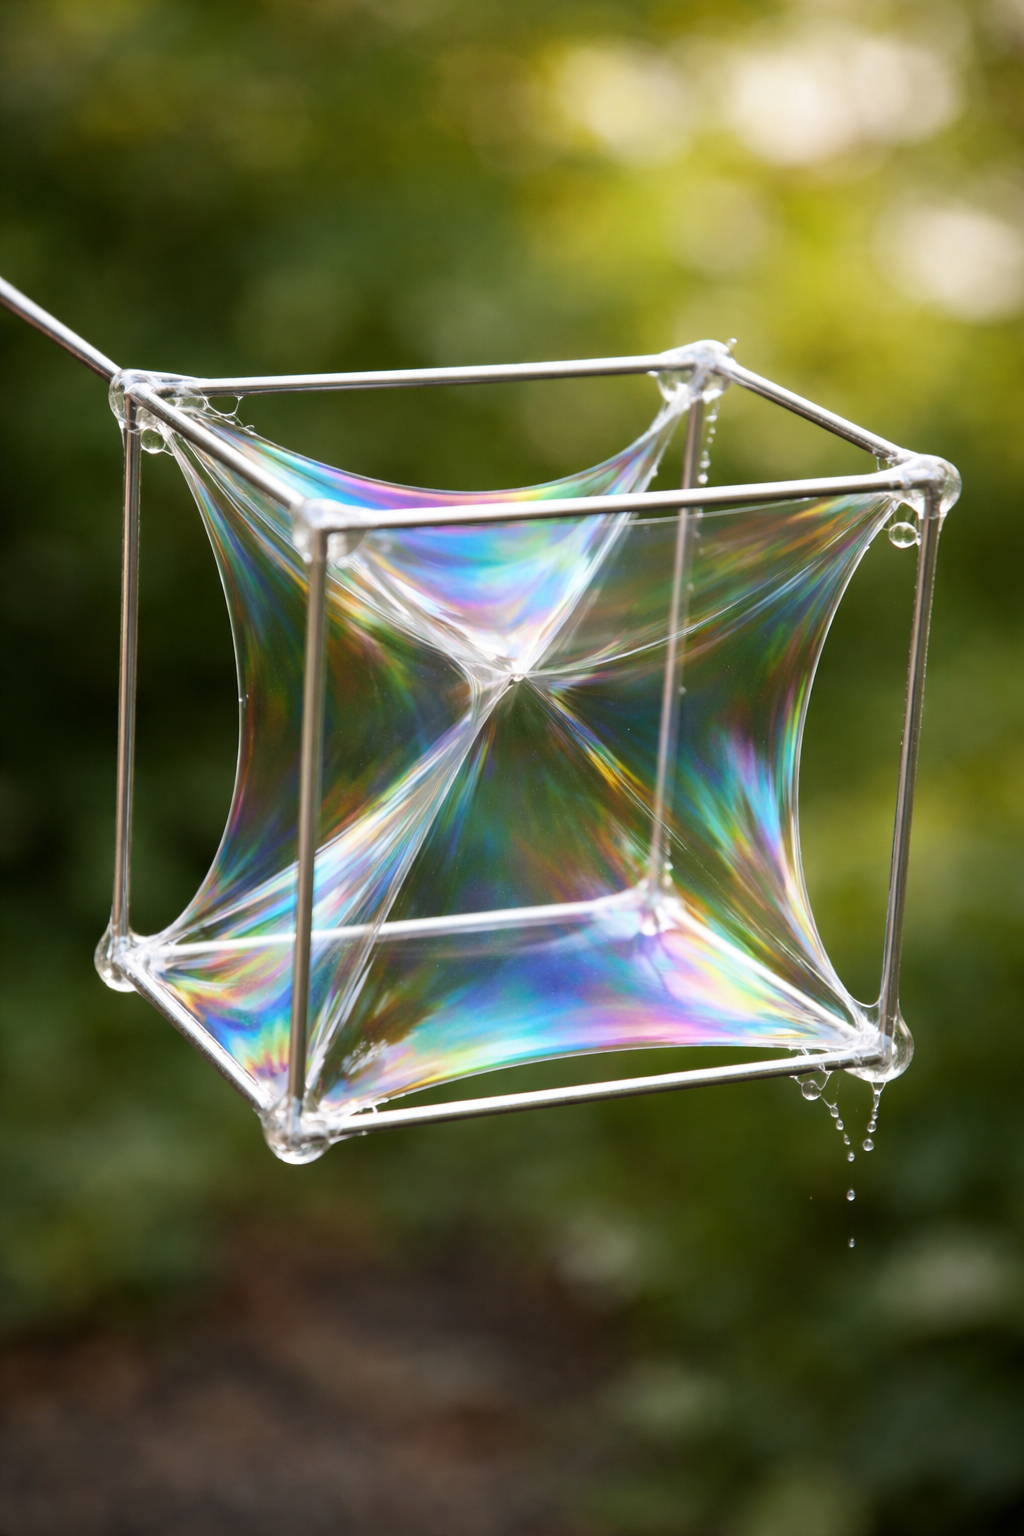
\includegraphics[width=0.62\linewidth]{bilder/seifenfilm.png}
	\caption{Seifenfilm in einem würfelförmigen Drahtrahmen. Die entstehende Form ist kein Zufall, sondern ergibt sich aus der Tendenz des Systems, unter gegebenen Randbedingungen eine möglichst kleine Oberfläche einzunehmen.}
	\label{fig:seifenfilm-drahtrahmen}
\end{figure}

\begin{NoteBox}[Warum der Seifenfilm diese Form annimmt]
	\small
	Die Oberfl\"achenspannung entsteht dadurch, dass sich die Wassermolek\"ule gegenseitig anziehen. An der Oberfl\"ache fehlen Nachbarn nach au{\ss}en, sodass dieser Zustand energetisch ung\"unstiger ist als im Inneren. Das System versucht deshalb, seine Oberfl\"ache m\"oglichst klein zu halten. Genau daraus entstehen unter gegebenen Randbedingungen die charakteristischen Minimalfl\"achen.
\end{NoteBox}

% =====================================================
% 10.6 Symmetrie in Kristallen und Schneeflocken
% =====================================================

\subsection{Symmetrie in Kristallen und Schneeflocken}
\index{Symmetrie}
\index{Kristall}
\index{Schneeflocke}
\index{Geometrie}
\index{Naturform}
\index{Struktur}

Symmetrie ist eines der auffälligsten Zeichen mathematischer Ordnung in der Natur. Wo immer Teile eines Objekts in bestimmter Weise wiederkehren, gespiegelt oder gedreht werden können, ohne dass die Grundform verloren geht, zeigt sich eine Struktur, die sich mathematisch präzise beschreiben lässt. Gerade in Kristallen und Schneeflocken tritt diese Ordnung besonders deutlich hervor.

Kristalle entstehen nicht in beliebiger Form. Ihre äußere Gestalt hängt mit der regelmäßigen Anordnung ihrer Bausteine im Inneren zusammen. Atome oder Moleküle ordnen sich in Gitterstrukturen, und diese innere Symmetrie prägt auch die äußere Form des Kristalls. Damit zeigt sich ein wichtiger Zusammenhang: Sichtbare Ordnung an der Oberfläche ist oft Ausdruck einer tieferen, unsichtbaren Ordnung im Inneren.

Ein besonders anschauliches Beispiel sind Schneeflocken. Sie erscheinen in unzähligen Varianten und doch besitzen sie fast immer eine sechsfache Grundsymmetrie. Diese Form geht auf die Struktur des Wassers und die Art zurück, wie sich Wassermoleküle beim Gefrieren anordnen. Die einzelnen Arme einer Schneeflocke wachsen unter ähnlichen Bedingungen, sodass eine gemeinsame Grundordnung erhalten bleibt. Zugleich führen kleine Unterschiede in Temperatur, Feuchtigkeit und Bewegung dazu, dass keine Schneeflocke der anderen vollkommen gleicht.

\begin{DidacticBox}[Symmetrie und Variation]
	Die mathematische Ordnung der Natur bedeutet nicht, dass alles vollkommen identisch sein muss. Gerade Schneeflocken zeigen, dass eine klare Grundsymmetrie mit individueller Vielfalt zusammenfallen kann. Struktur und Variation schließen einander nicht aus.
\end{DidacticBox}

Gerade darin liegt die mathematische Bedeutung solcher Formen. Symmetrie bedeutet nicht bloß Schönheit oder Regelmäßigkeit im ästhetischen Sinn. Sie zeigt an, dass unter bestimmten Transformationen etwas Wesentliches unverändert bleibt. In Kristallen und Schneeflocken ist diese Invarianz nicht von außen aufgeprägt, sondern wächst aus den physikalischen Bedingungen der Stoffe selbst hervor.

Für das Verständnis der Natur ist das von großer Bedeutung. Symmetrien erlauben es, komplizierte Formen auf wenige grundlegende Strukturprinzipien zurückzuführen. Sie machen sichtbar, dass hinter der Vielfalt der Erscheinungen oft einfache Ordnungen stehen. Mathematik erfasst diese Ordnungen nicht als bloße Dekoration, sondern als Ausdruck innerer Gesetzlichkeit.

Kristalle und Schneeflocken sind daher weit mehr als schöne Naturformen. Sie zeigen, dass die Welt nicht nur im Großen, sondern auch im Kleinen durch mathematisch beschreibbare Strukturen geprägt ist. Gerade in der Verbindung von Regel und Abweichung, von Symmetrie und individueller Ausprägung, wird sichtbar, wie tief mathematische Ordnung in die Natur hineinreicht.

\begin{figure}[htbp]
	\centering
	
\includegraphics[width=0.62\linewidth]{bilder/schneeflocke.png}
	\caption{Makroaufnahme einer Schneeflocke mit deutlich sichtbarer sechsf\"acher Symmetrie. Trotz individueller Unterschiede folgt ihre Grundform einer klaren geometrischen Ordnung, die aus der Struktur des Wassers und den Bedingungen des Kristallwachstums hervorgeht.}
	\label{fig:schneeflocke-symmetrie}
\end{figure}
\newpage
\noindent

% =====================================================
% 10.7 Musterbildung und Selbstorganisation
% =====================================================

\subsection{Musterbildung und Selbstorganisation}
\index{Musterbildung}
\index{Selbstorganisation}
\index{Ordnung}
\index{Natur}
\index{Reaktions-Diffusions-System}
\index{Dynamik}

Nicht alle mathematischen Strukturen der Natur sind von außen vorgegeben. Viele entstehen aus dem Zusammenspiel einfacher lokaler Prozesse, die ohne zentralen Plan zu geordneten Gesamtmustern führen. Genau dies bezeichnet man als \emph{Selbstorganisation}. Gemeint ist damit die Entstehung von Ordnung aus innerer Dynamik: Aus vielen kleinen Wechselwirkungen bildet sich eine größere Struktur, ohne dass diese Struktur von außen vollständig vorgegeben werden müsste.

Solche Prozesse finden sich in sehr unterschiedlichen Bereichen der Natur. Streifen und Flecken auf Tierfellen, Wellenmuster in Sanddünen, Rippenstrukturen auf Wasseroberflächen oder räumliche Muster in chemischen Reaktionen zeigen, dass Ordnung nicht immer das Ergebnis eines festen Bauplans ist. Oft genügt es, dass einfache Regeln lokal wirken und sich gegenseitig beeinflussen. Aus dieser Wechselwirkung entstehen Formen, die auf größerer Skala deutlich geordnet erscheinen.

Ein klassisches Beispiel sind sogenannte Reaktions-Diffusions-Systeme. Dabei breiten sich Stoffe im Raum aus, reagieren miteinander und beeinflussen sich wechselseitig. Schon aus wenigen Gleichungen können dadurch stabile Flecken, Streifen oder wellenartige Muster entstehen. Mathematisch ist daran besonders bemerkenswert, dass komplexe sichtbare Strukturen aus relativ einfachen Regeln hervorgehen k\"onnen.

\begin{DidacticBox}[Ordnung ohne zentralen Bauplan]
	Selbstorganisation bedeutet nicht Chaos, sondern geordnete Struktur aus lokaler Wechselwirkung. Ein Muster muss also nicht von außen entworfen werden. Es kann aus einfachen Regeln von selbst entstehen, wenn die Dynamik des Systems dies zulässt.
\end{DidacticBox}

Gerade darin liegt die tiefe mathematische Bedeutung solcher Phänomene. Mathematik beschreibt hier nicht nur eine fertige Form, sondern den Prozess ihrer Entstehung. Entscheidend ist nicht allein, wie ein Muster aussieht, sondern welche Gleichungen, Rückkopplungen und Stabilitätsbedingungen dazu führen, dass es sich ausbildet und erhalten bleibt. Die Ordnung liegt also nicht nur im Ergebnis, sondern im Gesetz der Dynamik selbst.

Zugleich zeigt sich an solchen Beispielen, dass mathematische Beschreibung weit über starre Geometrie hinausgeht. Mathematik erfasst nicht nur feste Formen wie Kreise, Sechsecke oder Kristalle, sondern auch Prozesse, in denen sich Struktur erst im Laufe der Zeit herausbildet. Gerade dadurch wird sichtbar, dass die Welt nicht nur geometrisch, sondern auch dynamisch mathematisch strukturiert ist.

Musterbildung und Selbstorganisation sind deshalb ein besonders starkes Beispiel f\"ur den Leitgedanken dieses Buches. Ordnung entsteht nicht nur dort, wo etwas von außen konstruiert wird, sondern auch dort, wo viele lokale Prozesse zusammenwirken. Mathematik macht diese verborgene Dynamik sichtbar und zeigt, dass selbst scheinbar spontane Naturformen oft einem präzise beschreibbaren Zusammenhang folgen.

Ein anschauliches Beispiel für Selbstorganisation liefern Dünenlandschaften. Auf den ersten Blick wirken Sanddünen wie bloße Formen der Natur. Tatsächlich entstehen sie jedoch aus einem dynamischen Zusammenspiel von Wind, Sandtransport, Ablagerung und Erosion. Kleine Unebenheiten im Sand verändern die Luftströmung, sodass an manchen Stellen mehr Material abgetragen und an anderen mehr abgelagert wird. Dadurch können sich kleine Störungen verstärken, bis aus zunächst unregelmäßigen Anfängen geordnete Wellen- und Dünenmuster entstehen.

Gerade hier zeigt sich, wo die mathematische Struktur der Selbstorganisation liegt. Sie steckt nicht nur in der fertigen Form, sondern vor allem in den Regeln ihrer Entstehung. Mathematik beschreibt in diesem Fall die Wechselwirkung lokaler Prozesse, die Rückkopplung zwischen Form und Strömung sowie die Bedingungen, unter denen aus kleinen Unregelmäßigkeiten stabile Muster hervorgehen. Ordnung entsteht also nicht trotz der Dynamik, sondern gerade aus ihr.

\begin{figure}[htbp]
	\centering
	
\includegraphics[width=0.82\linewidth]{bilder/duene.png}
	\caption{Dünenlandschaft mit windgeformten Sandrippen. Solche Muster entstehen nicht zufällig, sondern aus dem Zusammenspiel von Luftströmung, Sandtransport, Ablagerung und Rückkopplung. Die sichtbare Form ist Ausdruck eines dynamischen Prozesses mathematischer Selbstorganisation.}
	\label{fig:duene-selbstorganisation}
\end{figure}
\newpage
\noindent
\begin{DidacticBox}[Dünen als Beispiel für Selbstorganisation]
	Dünen zeigen, dass mathematische Struktur nicht nur in festen Formen liegt, sondern auch in den Regeln ihrer Entstehung. Wind, Sandtransport, Ablagerung und Rückkopplung entscheiden darüber, ob kleine Unebenheiten verschwinden oder zu einem geordneten Muster anwachsen.
\end{DidacticBox}

% =====================================================
% 10.8 Grenzen der Mathematisierung
% =====================================================
\subsection{Grenzen der Mathematisierung}
\index{Mathematisierung}
\index{Modell}
\index{Wirklichkeit}
\index{Grenze}
\index{Abstraktion}
\index{Naturbeschreibung}

So eindrucksvoll mathematische Strukturen in der Natur sichtbar werden, so wichtig ist auch eine nüchterne Einsicht: Nicht alles an der Wirklichkeit lässt sich vollständig in mathematische Form bringen. Mathematik ist ein außerordentlich mächtiges Erkenntnisinstrument, aber sie ist nicht mit der Wirklichkeit selbst identisch. Zwischen mathematischem Modell und konkreter Welt bleibt immer ein Unterschied bestehen.

Dieser Unterschied ist kein Mangel der Mathematik, sondern eine Folge ihres Wesens. Mathematik arbeitet mit Abstraktionen. Sie hebt bestimmte Beziehungen, Größen oder Strukturen hervor und lässt anderes bewusst weg. Gerade dadurch wird sie so stark. Ein Modell beschreibt nicht alles, sondern das Wesentliche im Hinblick auf eine bestimmte Fragestellung. Es gewinnt Klarheit durch Vereinfachung.

In der Natur ist jedoch kein System vollkommen ideal. Kein Kristall ist völlig fehlerfrei, kein Baum wächst exakt nach einem Lehrbuchschema, keine Düne ist nur das Ergebnis einer einzigen Gleichung. Zufällige Einflüsse, Störungen, historische Entwicklungen, Materialunterschiede und Wechselwirkungen mit der Umgebung führen dazu, dass reale Formen immer reicher und unregelmäßiger sind als ihre mathematischen Beschreibungen. Gerade deshalb darf man die mathematische Struktur nicht mit einer vollständigen Kopie der Wirklichkeit verwechseln.

\begin{DidacticBox}[Modell und Wirklichkeit]
	Ein mathematisches Modell ist keine Verdopplung der Welt. Es ist eine gezielte Beschreibung ihrer Struktur unter bestimmten Annahmen. Seine Stärke liegt nicht darin, alles zu erfassen, sondern das Wesentliche sichtbar zu machen.
\end{DidacticBox}

Diese Grenze bedeutet jedoch nicht, dass Mathematik nur ein beliebiges Hilfsmittel wäre. Im Gegenteil: Gerade weil sie abstrahiert, kann sie Ordnung, Gesetzmäßigkeit und Zusammenhänge sichtbar machen, die im unmittelbaren Eindruck verborgen bleiben. Ihre Reichweite ist groß, aber sie ist nicht grenzenlos. Sie zeigt Struktur, ohne die Wirklichkeit in ihrer ganzen Fülle zu erschöpfen.

Für ein verantwortliches Verständnis der Natur ist diese Unterscheidung entscheidend. Wer Mathematik überschätzt, verwechselt Modell und Welt. Wer sie unterschätzt, übersieht die Tiefe der Ordnung, die sich durch sie erkennen lässt. Die angemessene Haltung liegt zwischen beiden Extremen: Mathematik ist weder die vollständige Wirklichkeit noch bloß ein technisches Rechenwerkzeug. Sie ist das präziseste Mittel, das wir besitzen, um die Struktur der Welt zu erfassen, ohne deshalb mit der Welt selbst identisch zu sein.

Gerade an dieser Grenze zeigt sich erneut ihre philosophische Bedeutung. Mathematik ist stark, weil sie abstrahiert. Sie ist erfolgreich, weil sie vereinfacht. Und sie bleibt glaubwürdig, wenn sie ihre eigenen Grenzen kennt. So bestätigt sich auch hier der Leitgedanke dieses Buches: Die Welt ist mathematisch strukturiert, aber sie fällt nicht restlos mit ihrem mathematischen Bild zusammen.
Ein anschauliches Beispiel liefert die Bruchmechanik. Bei einer belasteten Metallplatte lassen sich Spannungen, Materialeigenschaften und kritische Belastungsgrenzen mathematisch beschreiben. Dennoch ist der genaue Zeitpunkt oder Verlauf eines realen Risses oft nur schwer vorherzusagen. Schon kleinste Materialfehler, Einschlüsse, Mikrorisse oder Unregelmäßigkeiten in der Belastung können darüber entscheiden, wo ein Riss entsteht und wie er sich ausbreitet. Gerade daran zeigt sich die Grenze der Mathematisierung: Die Struktur des Problems ist mathematisch erfassbar, aber die konkrete Wirklichkeit bleibt oft empfindlich gegenüber Details, die sich nicht vollständig kontrollieren lassen.
\begin{figure}[htbp]
	\centering
	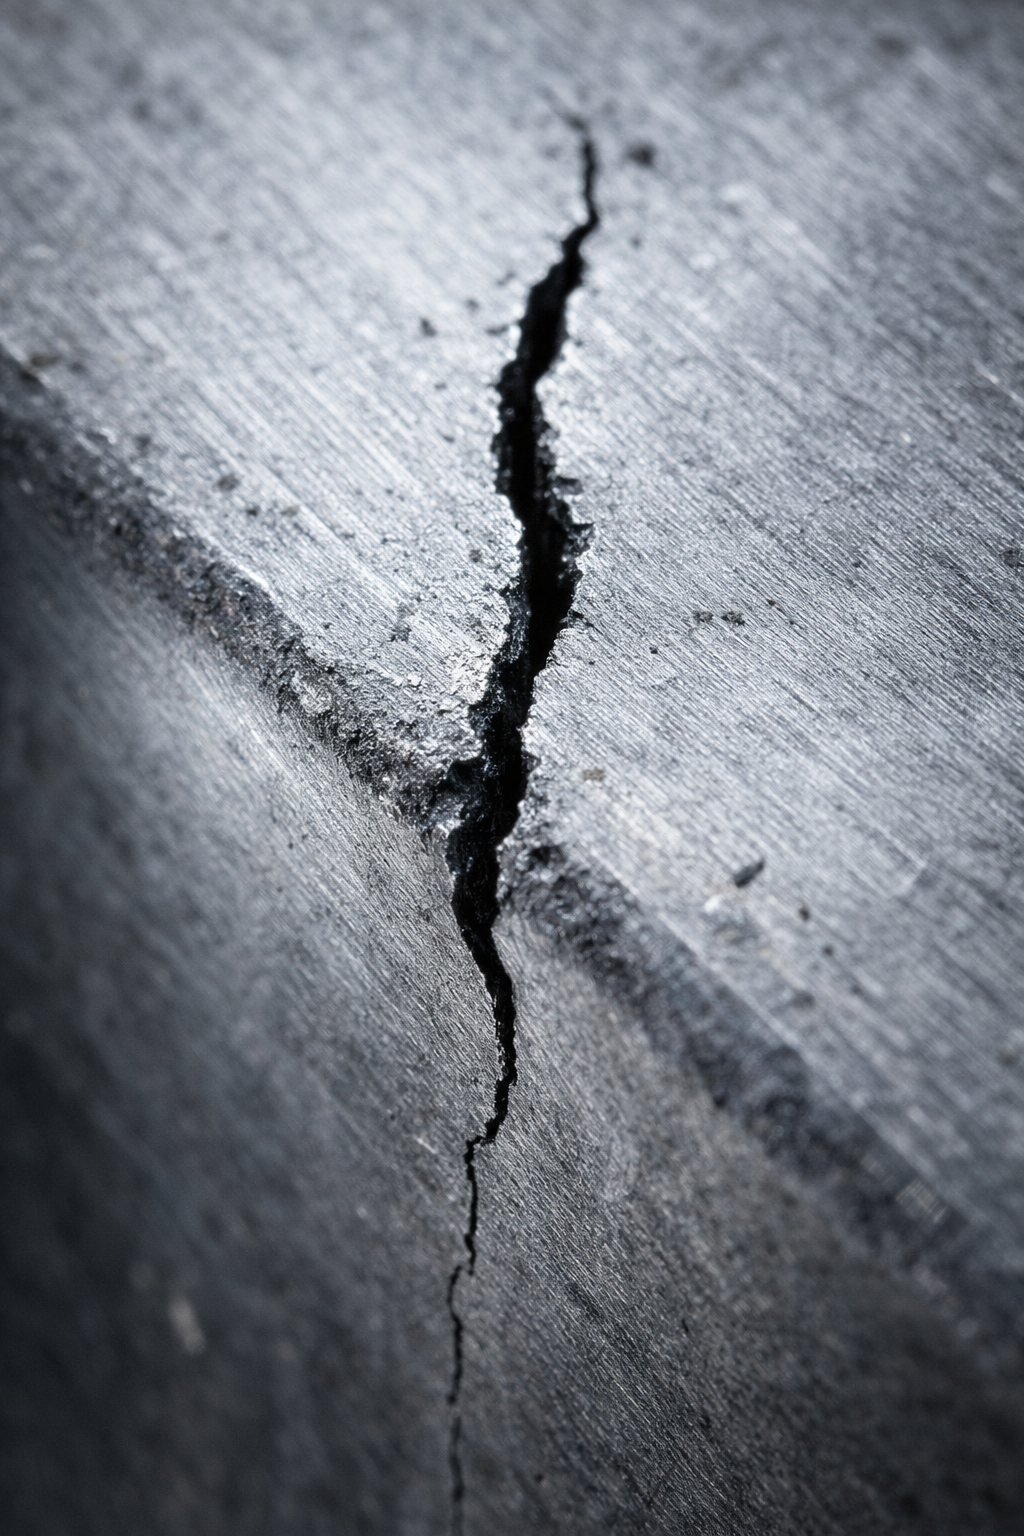
\includegraphics[width=0.62\linewidth]{bilder/haarriss.png}
	\caption{Haarriss in einer belasteten Metalloberfläche. In vielen Fällen entsteht ein solcher Riss nicht schlagartig, sondern durch langsame Materialermüdung. Über lange Zeit wachsen mikroskopische Schädigungen, bis schließlich ein sichtbarer Riss auftritt. Gerade daran zeigt sich, dass mathematische Modelle die Struktur des Problems erfassen können, während der konkrete Zeitpunkt und Verlauf in der Realität oft schwer vorherzusagen bleiben.}
	\label{fig:metallriss-haarriss}
\end{figure}
\newpage
\noindent
\begin{DidacticBox}[Grenze mathematischer Vorhersage]
	Dass ein Vorgang mathematisch beschreibbar ist, bedeutet nicht, dass jedes reale Einzelereignis exakt vorhergesagt werden kann. Gerade bei empfindlichen Systemen können kleinste Materialunterschiede oder Störungen den konkreten Verlauf entscheidend beeinflussen.
\end{DidacticBox}

% =====================================================
% 10.9 Fazit: Natur als mathematische Struktur
% =====================================================

\subsection{Fazit: Natur als mathematische Struktur}

Die Beispiele dieses Kapitels haben gezeigt, dass Mathematik in der Natur nicht nur in abstrakten Formeln oder idealisierten Figuren vorkommt. Sie tritt in realen Formen, Wachstumsprozessen und Ordnungen hervor: in den Waben des Bienenstocks, in den Verzweigungen eines Baumes, in Spiralen von Pflanzen, in den Minimalflächen von Seifenhäuten, in der Symmetrie von Schneeflocken und in der Selbstorganisation von Dünenlandschaften. Überall zeigt sich, dass die sichtbare Welt nicht bloß vielfältig, sondern in vielen Fällen auch mathematisch strukturiert ist.

Dabei bedeutet mathematische Struktur nicht, dass die Natur wie ein starres Lehrbuch aufgebaut wäre. Reale Systeme bleiben unvollkommen, gestört und von vielen Einflüssen geprägt. Gerade deshalb liegt die Stärke der Mathematik nicht in der exakten Verdopplung der Wirklichkeit, sondern in der Fähigkeit, unter wechselnden Bedingungen die tragenden Ordnungsprinzipien sichtbar zu machen. Sie zeigt nicht jedes Detail, aber sie macht verständlich, warum bestimmte Formen bevorzugt auftreten, warum Wachstum bestimmten Mustern folgt und warum sich unter gegebenen Bedingungen gerade einige Strukturen als stabil, effizient oder energetisch günstig erweisen.

Damit gewinnt auch die Grundidee dieses Buches neue Anschaulichkeit. Mathematik ist nicht nur ein Werkzeug des menschlichen Denkens, das nachträglich auf die Welt angewandt wird. Sie ist vielmehr das Mittel, mit dem wir die Ordnung erkennen, die in der Welt selbst wirksam ist. Die Natur ist nicht mathematisch dekoriert, sondern mathematisch strukturiert.

Gerade darin liegt die tiefere Bedeutung der hier betrachteten Beispiele. Sie zeigen, dass mathematische Formen nicht nur in der Theorie, sondern in der Wirklichkeit auftreten -- nicht immer vollkommen, nicht immer ideal, aber doch so deutlich, dass ihre Struktur erkennbar wird. Von der Zahl über die Geometrie bis zur Dynamik bestätigt sich immer wieder derselbe Gedanke: Die Welt ist nicht bloß vorhanden, sondern geordnet. Und Mathematik ist die Sprache und Erkenntnisform dieser Ordnung.